% !TeX root = ../thoulon_phd_defense_2025.tex
\documentclass[beamer]{standalone}
% \documentclass[../thoulon_phd_defense_2025.tex]{subfiles}

% \graphicspath{{\subfix{../chapters/}}}
\begin{document}

\section[Baseline]{Baseline geometry}
\subsection{Geometry}
\begin{frame}
    \frametitle{Generic Fighter Aircraft (GFAs)}
	No air intake, canard or empenage.% Ledge at the front of the fuselage.


    \begin{figure}[htb]
		\centering
		\captionsetup[subfigure]{justification=centering}
		\begin{subfigure}[c]{0.66\textwidth}
			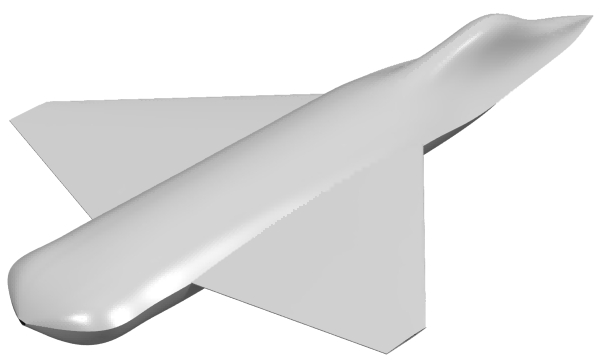
\includegraphics[width=.8\textwidth]{images/gfa/baseline-view.jpg}
			% 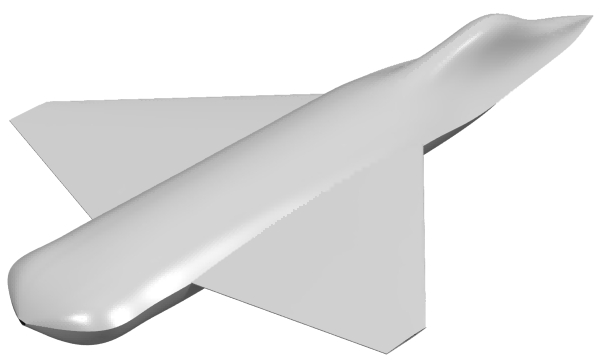
\includegraphics[width=.9\textwidth,center]{images/gfa/baseline-view.jpg}
			\caption*{3D-view.}
		\end{subfigure}
		\begin{subfigure}[c]{0.33\textwidth}
			\centering
			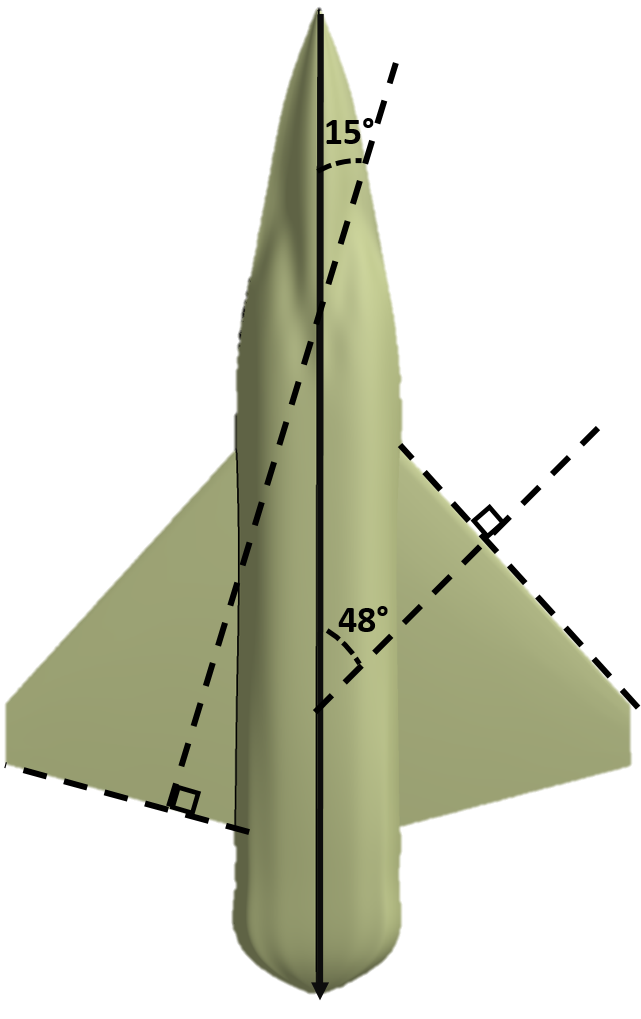
\includegraphics[width=.8\textwidth]{images/gfa/base-shape.png}
			% 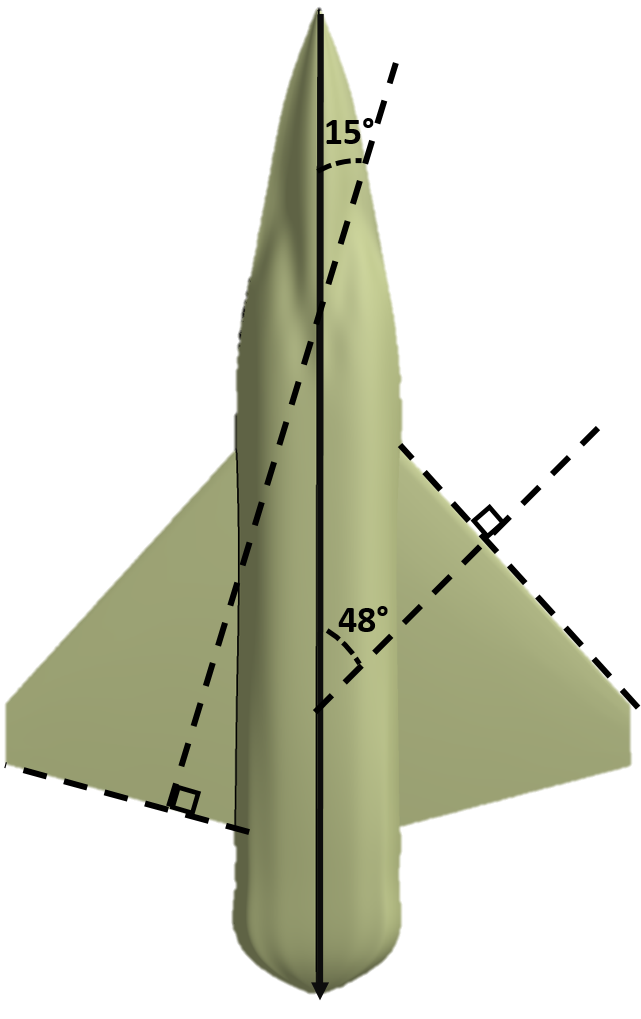
\includegraphics[width=.9\textwidth,center]{images/gfa/base-shape.png}
			\caption*{Bottom view with the leading and trailing edge sweep angles.}
		\end{subfigure}
		\caption*{The Generic Fighter Aircraft.}
		\label{fig:baseline-model}
	\end{figure}
\end{frame}

\begin{frame}
	\frametitle{Angle definition}

	\begin{figure}
		\centering
		\resizebox{!}{.5\textheight}{
		\subimport{resources/intro/}{def-angles.tex}
		}
		\caption*{Definition of the bearing ($\color{blue} \theta$) and elevation ($\color{red} \phi$) angles.}
	\end{figure}

\end{frame}

\subsection{RCS analysis}
\begin{frame}
    \frametitle{RCS Analysis}
	The RCS is mainly conscentrated in two directions : 48$^\circ$ (specular reflexion on the leading edge) and 15$^\circ$ (diffraction on the trailing edge). It is very small elsewhere.
	\begin{figure}
		\centering
		\captionsetup[subfigure]{justification=centering}
		\begin{subfigure}{.49\textwidth}
            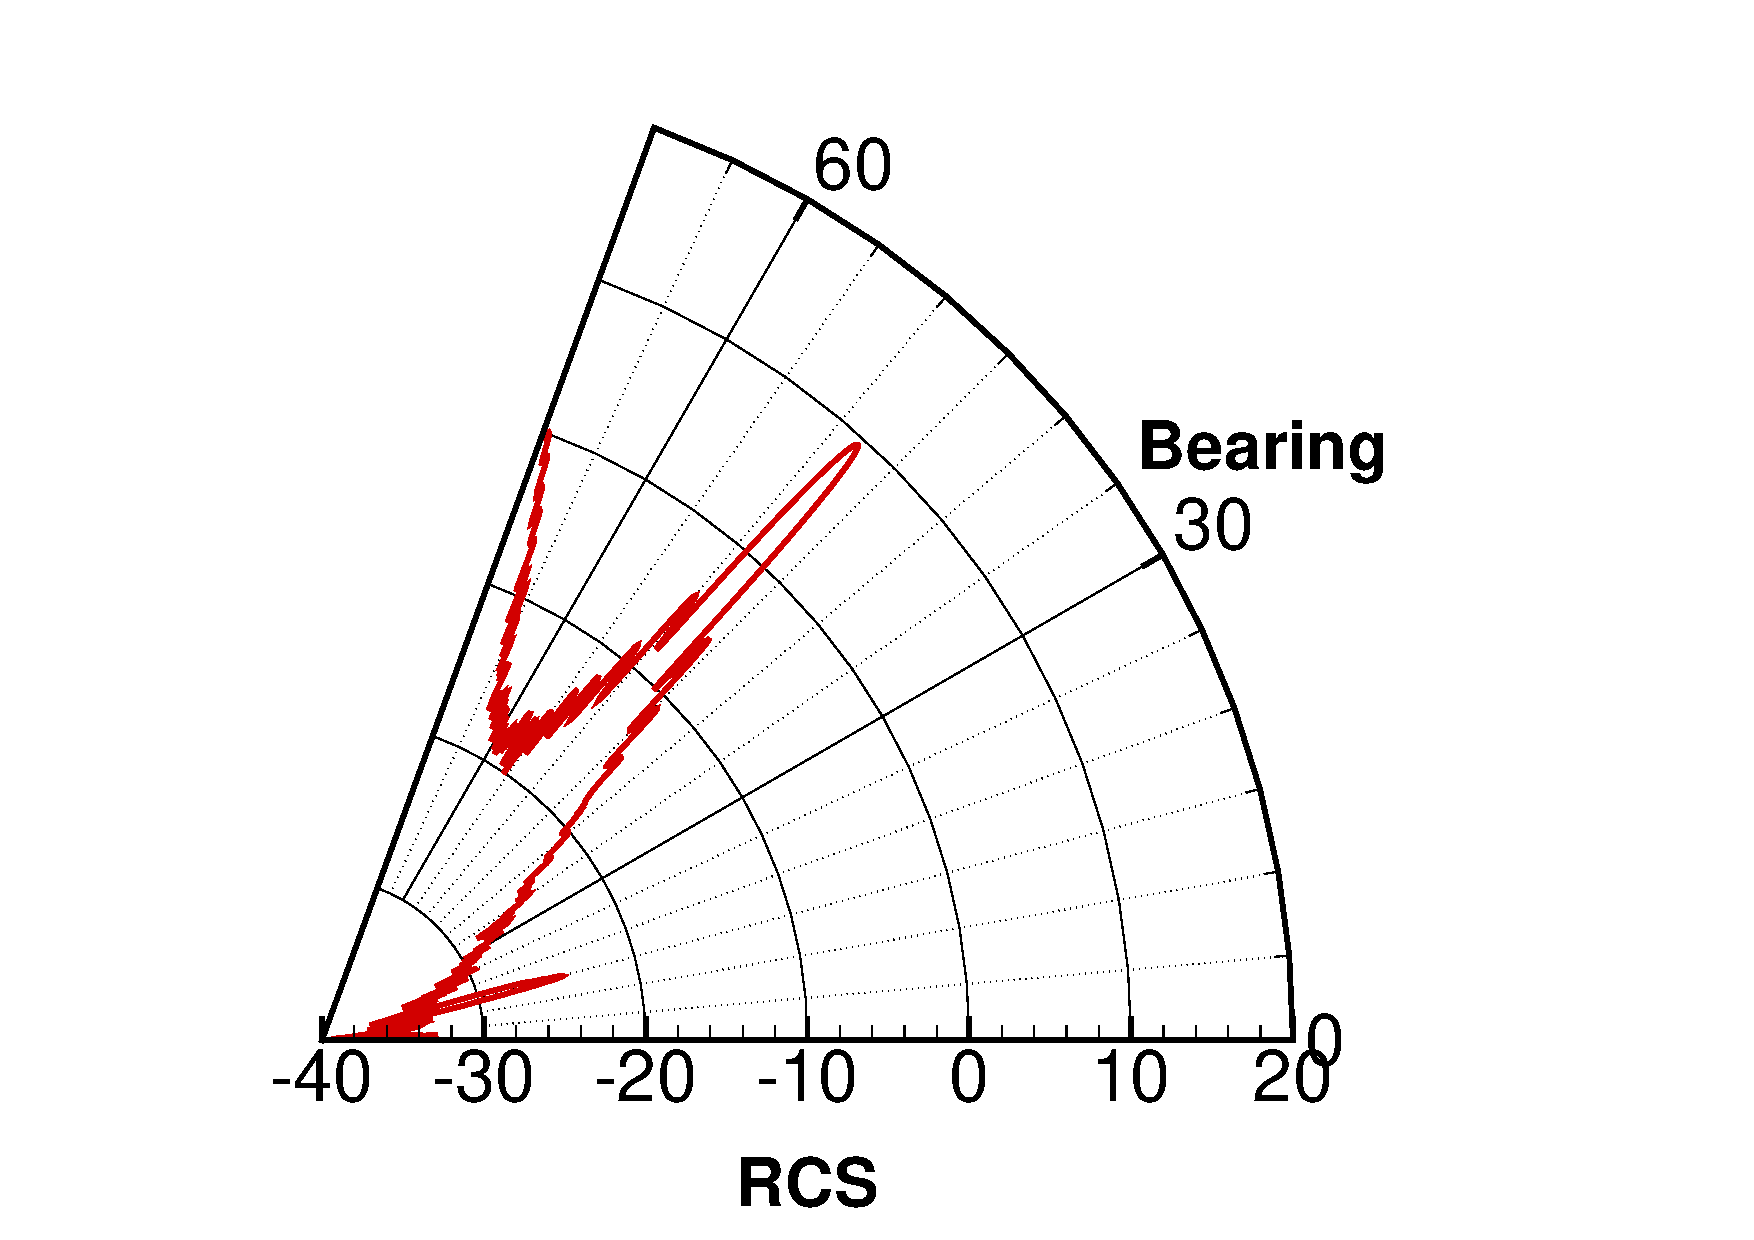
\includegraphics[trim={5cm .5cm 5cm 2cm}, clip,width=.8\textwidth,height=0.8\textheight,keepaspectratio,center]{images/gfa/PO-PH-PTD.pdf}
            \vspace*{-4ex}
            \caption*{\scriptsize Horizontal polarization.}
		\end{subfigure}
		\begin{subfigure}{.49\textwidth}
			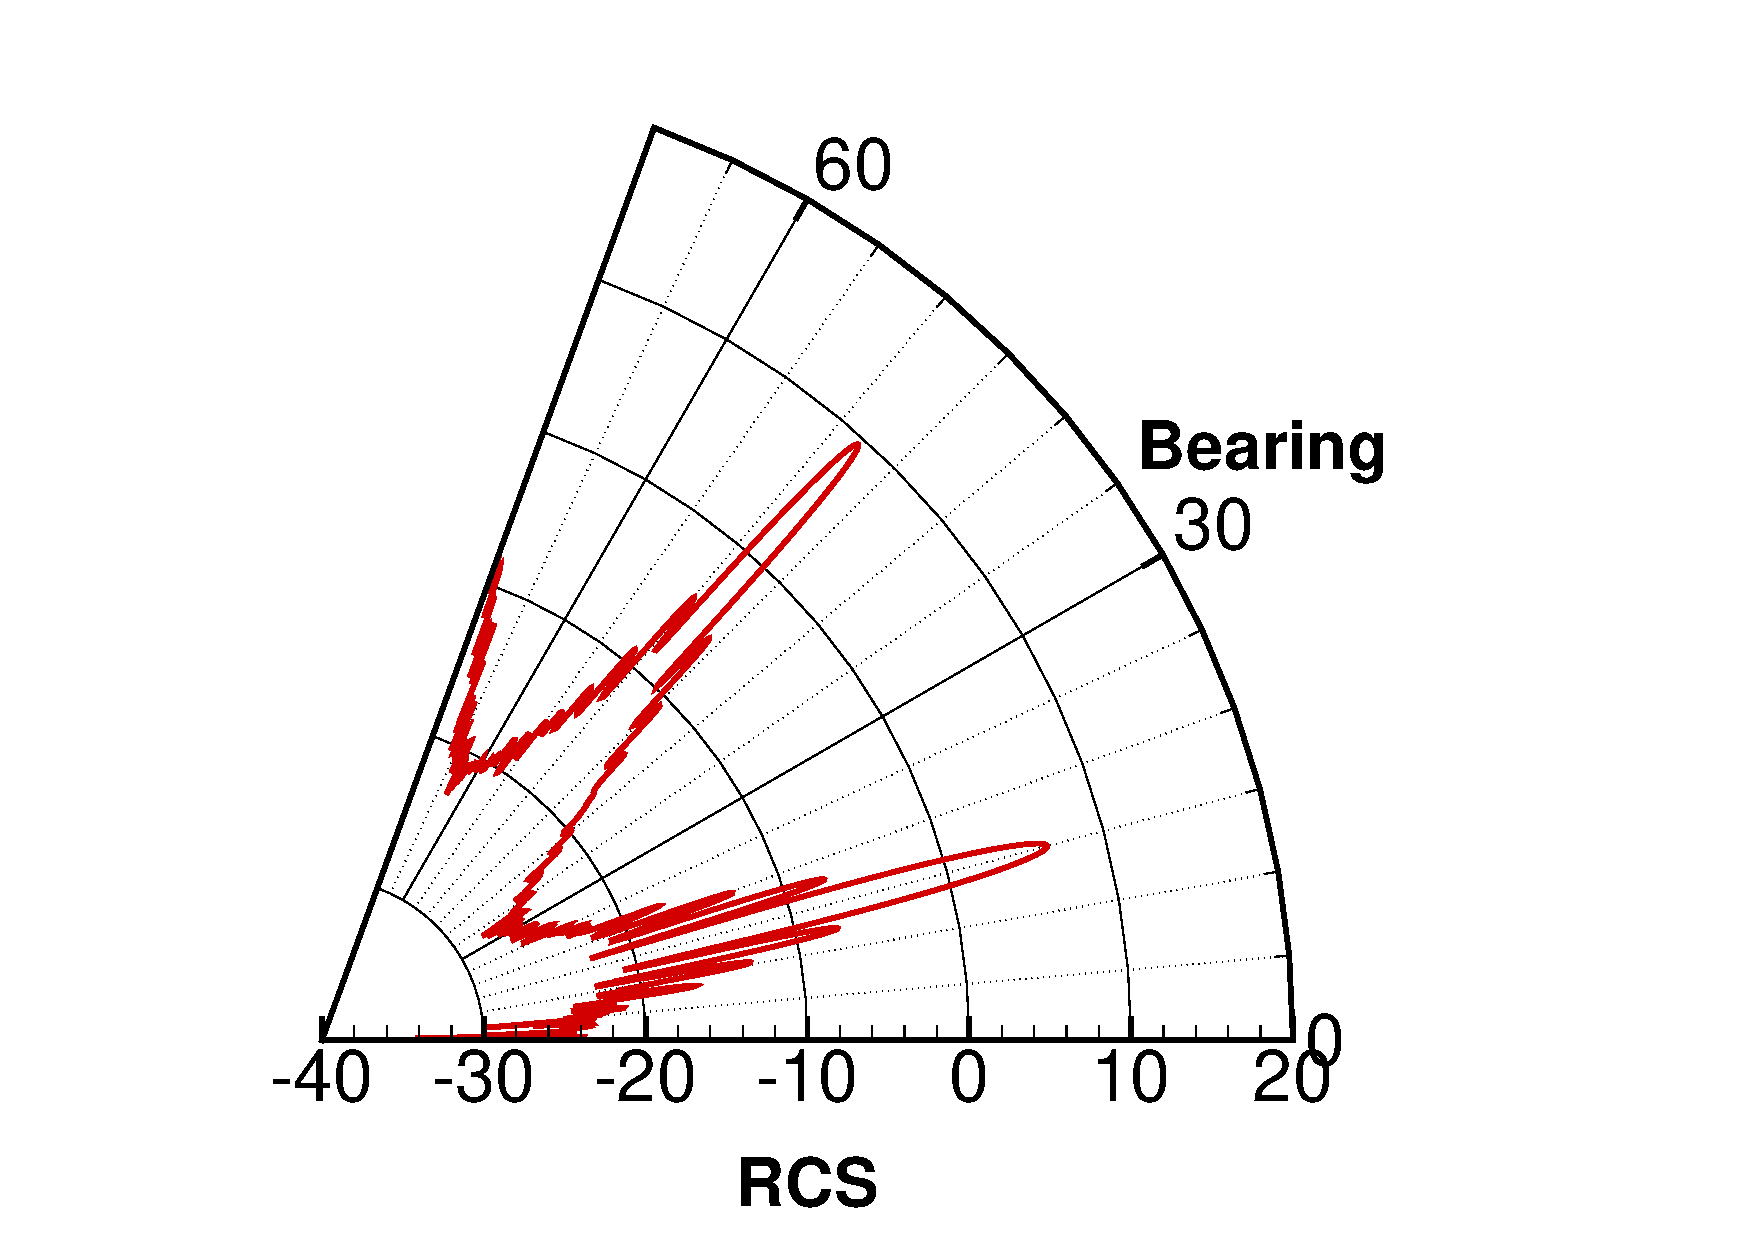
\includegraphics[trim={5cm .5cm 5cm 2cm}, clip,width=.8\textwidth,height=.8\textheight,keepaspectratio,center]{images/gfa/PO-PV-PTD.pdf}
            \vspace*{-4ex}
			\caption*{\scriptsize Vertical polarization.}
		\end{subfigure}
		\onslide<1->
        \vspace*{-1ex}
		\caption*{\small Profile of RCS with respect to the bearing angle on the GFA (elevation: $-20^\circ$, $f = 2\unit{\giga\hertz}$).}
    \end{figure}
	% \begin{figure}
	% 	\centering
	% 	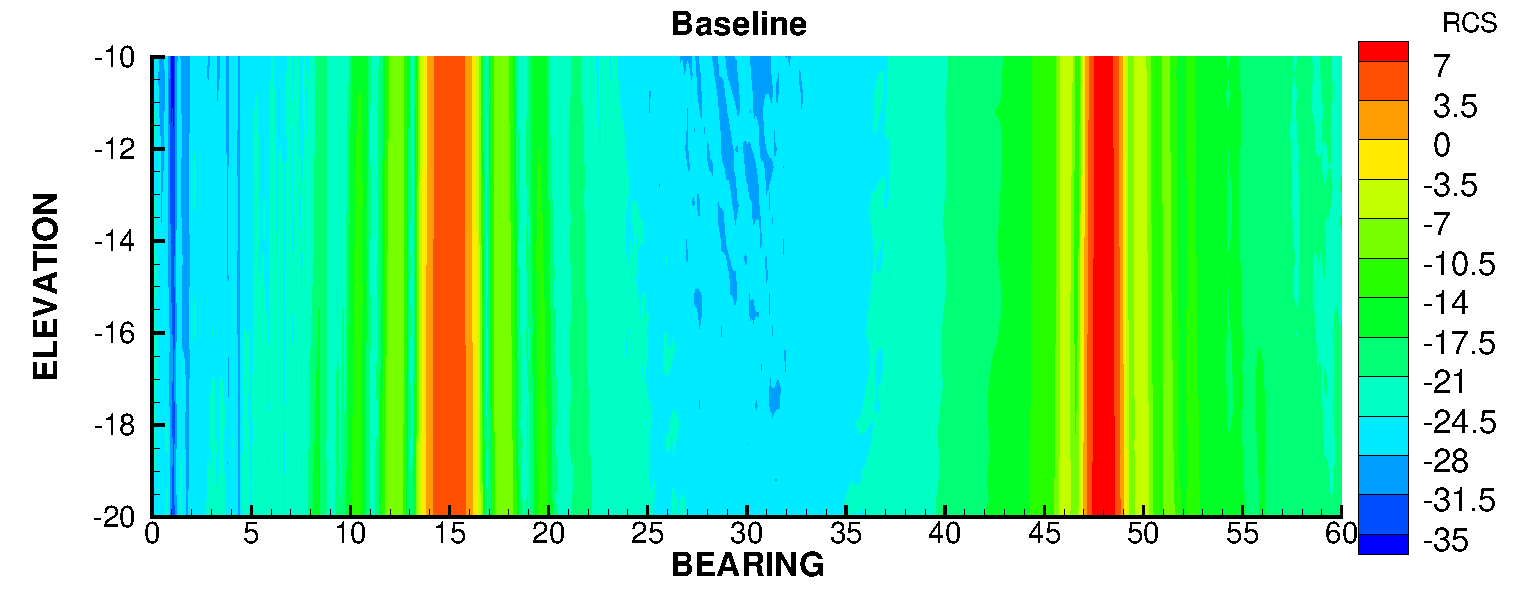
\includegraphics[width=1\textwidth, height=.75\textheight, keepaspectratio]{images/gfa/RCS_RCS_baseline.pdf}
	% 	\caption*{RCS of the baseline GFA at $f = 2 \unit{\giga\hertz}$ (vertical polarization)}
	% \end{figure}
\end{frame}

\subsection{Aerodynamic analysis}
\begin{frame}
	\frametitle{Aerodynamic analysis - wing cross-section}
	A weak shock develops around the wing leading edge.
	\begin{figure}[htp]
		\centering
		\captionsetup{justification=centering}
		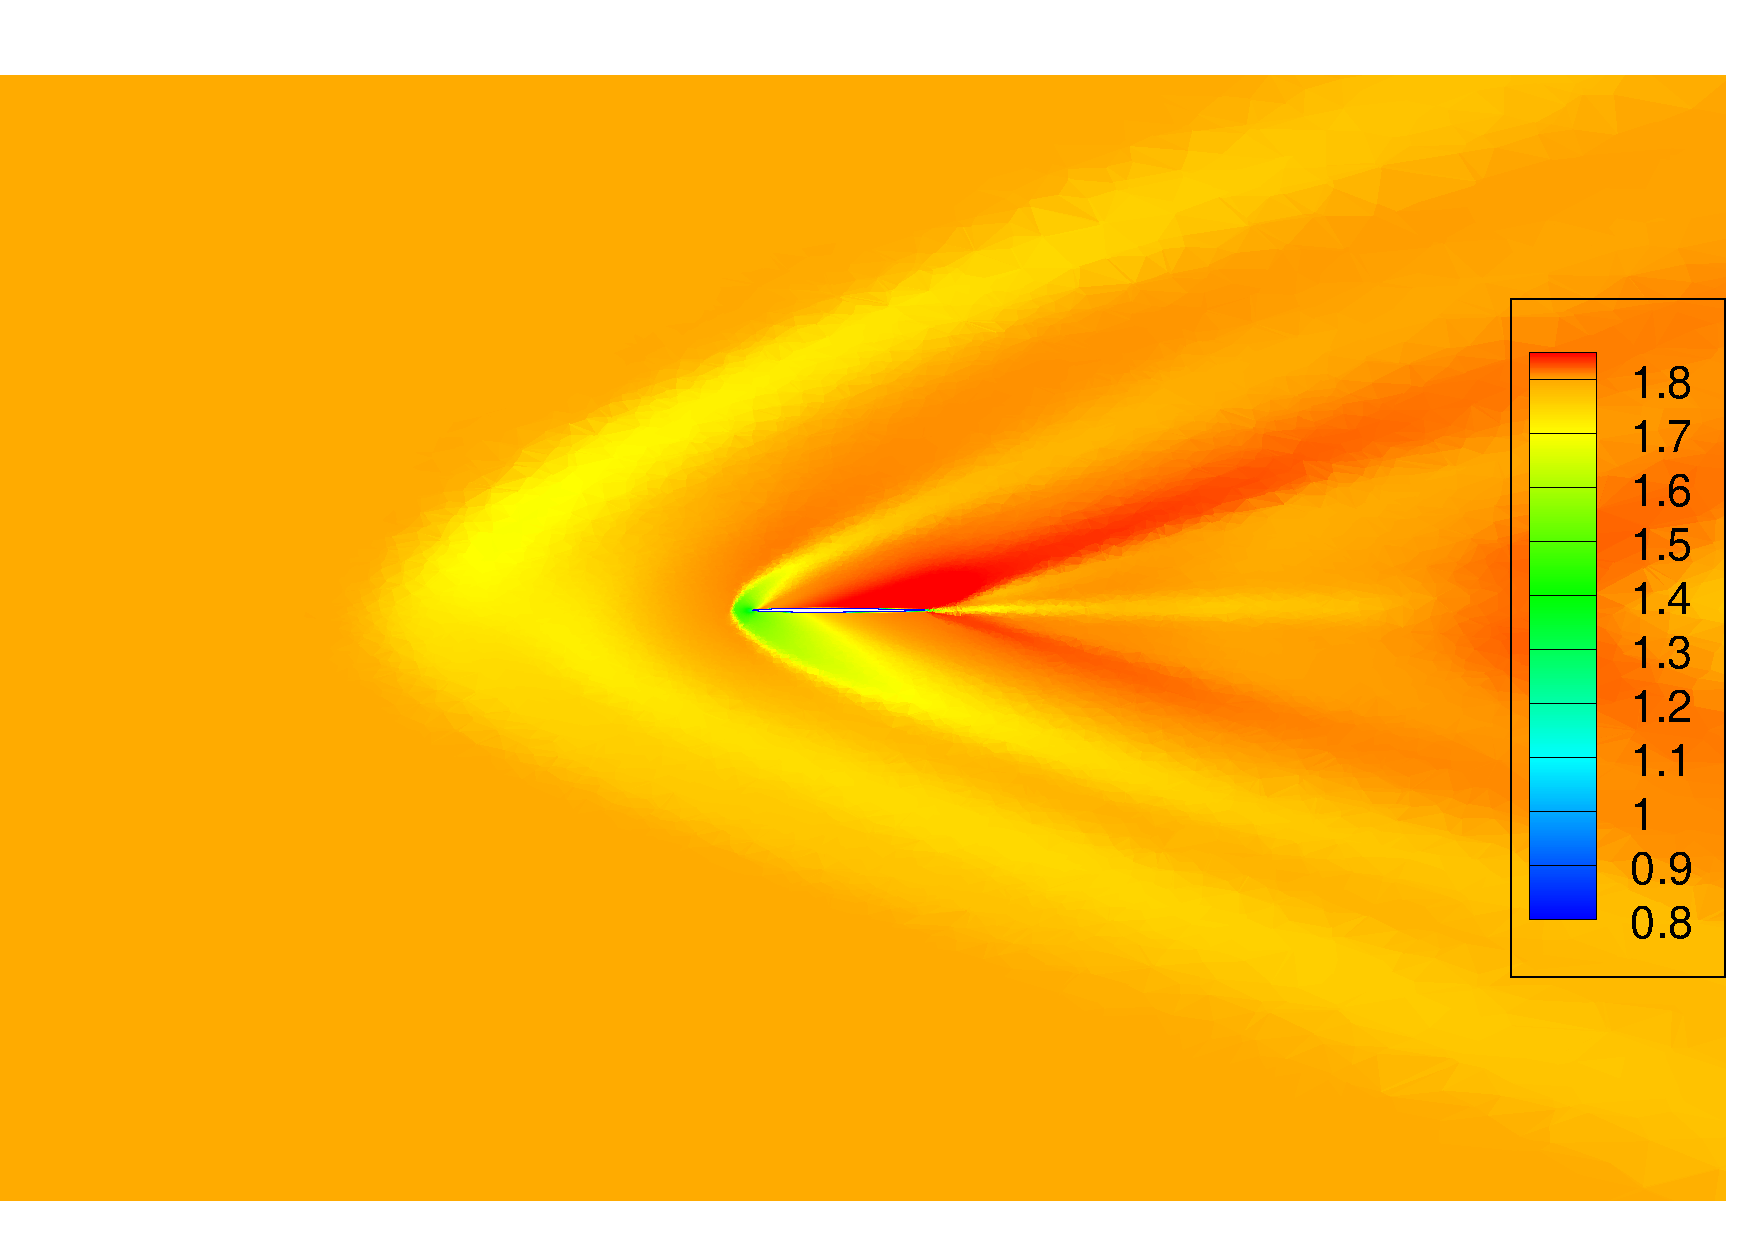
\includegraphics[width=0.75\textwidth]{images/gfa/MALO_5_ref.pdf}
		\caption*{Distribution of local Mach number around the cross-section of the wing of the GFA, at $Y/b = 0.8$.}
		\label{bidis-fig:MALO-5-baseline}
	\end{figure}
\end{frame}

\begin{frame}
    \frametitle{Paramétrisation}
    \begin{figure}[htb]
		\centering
		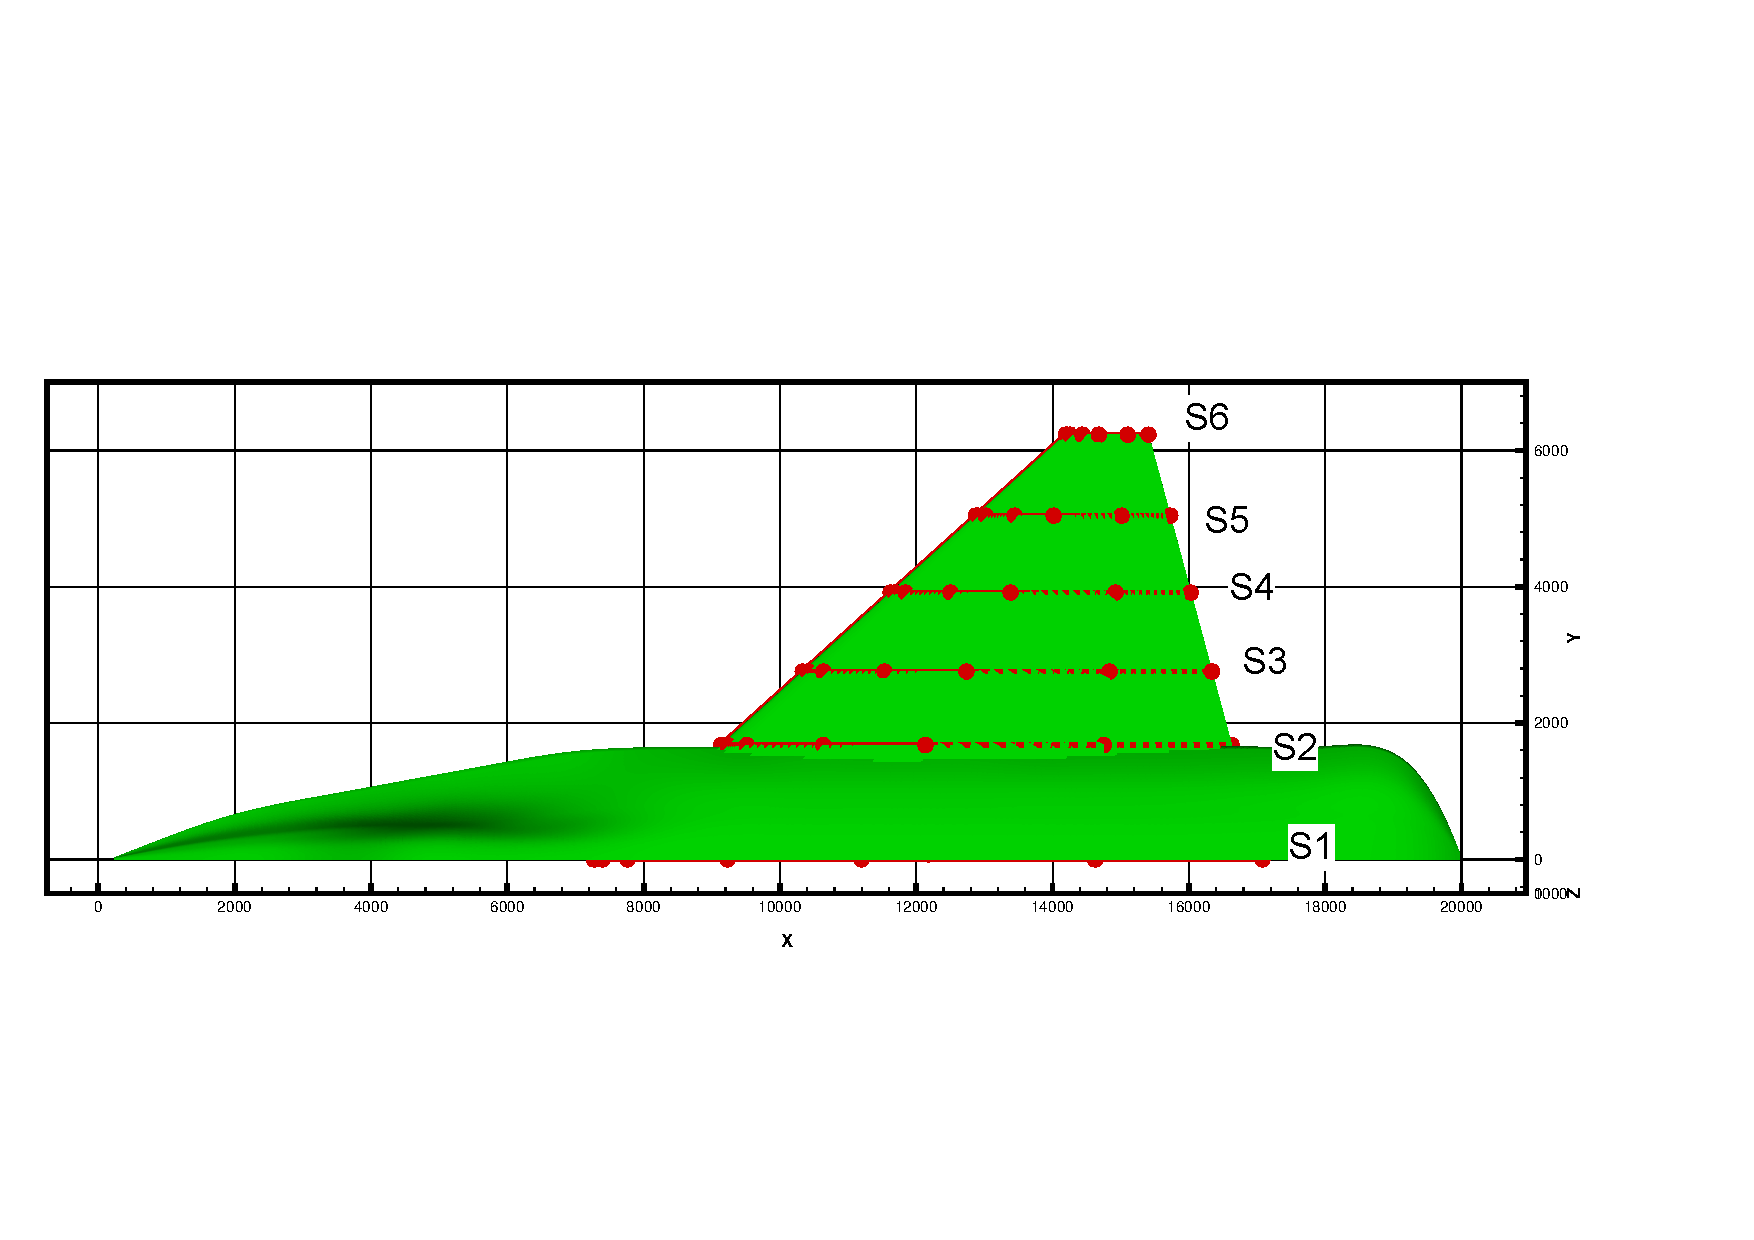
\includegraphics[trim=5mm 45mm 20mm 55mm,clip,width=\textwidth,height=.4\textheight,keepaspectratio]{images/gfa/control_sections-h.pdf}
		% \frame{\includegraphics[trim=100mm 0 115mm 0mm,clip,width=.75\textwidth]{control_sections-v.pdf}}
		% \caption*{The wing parametrized with the control sections and control points.}
		\label{fig:parametrized-shape}
	\end{figure}%
    \only<1>{%
	The GFA wing is parameterized with 6 control sections, 15 control points along each section. The geometry is interpolated between the control sections using RBF.
    }%
    \onslide<2->
	The geometry is parameterized with 13 global variables :
	\begin{itemize}[label=\ding{227}]
		\item<3-> leading edge sweep angle at sections 2 and 4,
		\item<4-> chord length of sections 2, 4 and 6,
		\item<5-> distance between sections 2 and 6 (span),
		\item<6-> twist angle at sections 2, 3 ,5 and 6,
		\item<7-> leading edge camber at sections 3, 5 and 6.
	\end{itemize}
    \onslide<8->
	The aerodynamic angle of attack is the \nth{14} optimization parameter (useful only for aerodynamic optimization).
\end{frame}
\end{document}